\documentclass[12pt]{article}

\usepackage{sbc-template}
\usepackage[brazil,american]{babel}
\usepackage[utf8]{inputenc}

\usepackage{graphicx}
\usepackage{url}
\usepackage{float}
\usepackage{listings}
\usepackage{color}
\usepackage{todonotes}
\usepackage{algorithmic}
\usepackage{algorithm}
\usepackage{hyperref}
\usepackage{indentfirst}
\usepackage{longtable}
\usepackage[inline]{enumitem}


\graphicspath{{./images/}}

\sloppy

\title{Laboratório 4\\- CPU MIPS Multiciclo –}

\author{GRUPO 6\\
	Dayanne Fernandes da Cunha, 13/0107191\\
	Lucas Mafra Chagas, 12/0126443\\
	Marcelo Giordano Martins Costa de Oliveira, 12/0037301\\
	Lucas Junior Ribas, 16/0052289\\
	Caio Nunes de Alencar Osório, 16/0115132\\
	Diego Vaz Fernandes, 16/0117925}

\address{Dep. Ciência da Computação -- Universidade de Brasília (UnB)\\
  CiC 116394 - OAC - Turma A
  \email{}
}

\begin{document}
\maketitle

\section{Objetivos}
\label{sec:Objetivos}

\begin{itemize}
\item Treinar o aluno com a linguagem de descrição de \textit{hardware} \textit{Verilog};
\item Familiarizar o aluno com a plataforma de desenvolvimento \textit{FPGA DE2} da \textit{Altera} e o software \textit{QUARTUS II};
\item Desenvolver a capacidade de análise e síntese de sistemas digitais usando uma Linguagem de Descrição de \textit{Hardware};
\item Apresentar ao aluno a implementação de uma \textit{CPU MIPS Multiciclo}.
\end{itemize}

\section{Ferramentas}
\label{sec:Materiais}

Todos os códigos escritos neste laboratório podem ser encontrados no repositório \url{https://github.com/Dayof/OAC172} do \textit{GitHub}.

\begin{itemize}
\item FPGA DE2 da Altera 
\item QUARTUS-II
\item Verilog HDL
\end{itemize}

\section{Exercício 2. Análise do processador Multiciclo}
\label{sec:multiciclo}


\section{Exercício 3. Teste do funcionamento das instruções da \textit{ISA} }
\label{sec:testeisa}


\section{Exercício 4. Software de lançamento de bola de canhão na \textit{FPGA}}
\label{sec:canhao}


\section{Exercício 5. Demonstração dos cenários}
\label{sec:cenarios}

  
\section{Exercício 6. Novas instruções usando a \textit{ISA MIPS}}
\label{sec:isamips}

Na Tabela~\ref{tab:mul} mostra a instrução \textit{MUL} do tipo R que foi inserida na \textit{ISA MIPS} Multiciclo.

\begin{table}[H]
	\centering
	\begin{tabular}{|c|c|c|c|c|c|c|}
		\hline
		INSTRUÇÃO & OPCODE (6) & RS (5) & RT (5) & RD (5) & SHAMT (5) & FUNCT (6) \\\hline
		MUL \$t1, \$t2, \$t3 & 000000 & x & x & x & 00000 & 000010 \\\hline
	\end{tabular}
	\caption{Componentes da instrução \textit{MUL}.}
	\label{tab:mul}
\end{table}

Para preencher a Tabela~\ref{tab:mul} foi usada a informação que as instruções do tipo R sempre possuem o \textit{OPCODE} em zero. A ordem dos componentes de \textit{MUL} é \textit{MUL RD RS RT}. \textit{RS} e \textit{RT} se referem aos argumentos da operação, no caso, \$t2 e \$t3 respectivamente e \textit{RD} para o registrador destino, ou seja, \$t1. Como \textit{MUL} não é uma instrução que usa operações \textit{SHIFT} então este campo também permanece com zeros. O componente \textit{FUNCT} foi preenchido de acordo com a fonte \cite{mips32}.

Na Tabela~\ref{tab:mul} mostra a instrução \textit{JALR} do tipo R que foi inserida na \textit{ISA MIPS} Multiciclo.

\begin{table}[H]
	\centering
	\begin{tabular}{|c|c|c|c|c|c|c|}
		\hline
		Instrução & OPCODE (6) & RS (5) & RT (5) & RD (5) & SHAMT (5) & FUNCT (6) \\\hline
		JALR \$t1 & 000000 & x & 00000 & 11111 & 00000 & 001001 \\\hline
		JALR \$t1, \$t2 & 000000 & x & 00000 & x & 00000 & 001001 \\\hline
	\end{tabular}
	\caption{Componentes da instrução \textit{JALR}.}
	\label{tab:jalr}
\end{table}

Para preencher a Tabela~\ref{tab:jalr} também foi usada a informação que as instruções do tipo \textit{R} sempre possuem o \textit{OPCODE} em zero. A ordem dos componentes de \textit{JALR} é \textit{JALR RD RS}. Na instrução com apenas \textit{\$t1} o componente \textit{RD} é preenchido com 11111 para representar o \textit{\$ra}. Em ambas instruções da Tabela~\ref{tab:jalr} o componente \textit{RT} não é utilizado. E como \textit{JALR} não é uma instrução que usa operações \textit{SHIFT} então este campo também permanece com zeros. O componente \textit{FUNCT} foi preenchido de acordo com a fonte \cite{mips32}.

Para implementar estas instruções os arquivos \textit{Parametros.v}, \textit{ALUControl.v}, \textit{Datapath\_MULT.v} e \textit{Control\_MULT.v} foram modificados. 

\subsection{Parêmetros}
\label{subsec:param}

O \textit{OPCODE} de \textit{MUL} e \textit{JALR} não precisam de nenhuma adição no arquivo já que são do tipo R.

Os componentes \textit{FUNCT} foram adicionados no arquivo como é mostrado na Figura~\ref{fig:pfunct}.

\begin{figure}[H]
	\flushleft
	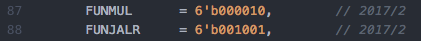
\includegraphics[width=1\textwidth]{pfunct.png}
	\caption{Parâmetros para o componente \textit{FUNCT} de cada instrução.}
	\label{fig:pfunct}
\end{figure}

Os parâmetros para a máquina estado do multiciclo foram adicionados conforme a Figura~\ref{fig:pest}.

\begin{figure}[H]
	\flushleft
	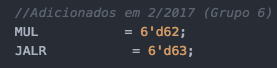
\includegraphics[width=1\textwidth]{pest.png}
	\caption{Parâmetros para a máquina de estados multiciclo.}
	\label{fig:pest}
\end{figure}

A operação \textit{MUL} não foi adicionada no arquivo pois o \textit{OPMULT} implementada no arquivo \textit{ALU.v} já implementa o resultado esperado para \textit{MUL}. No caso seria colocar em \textit{HI} e \textit{LO} o resultado da operação \textit{iA * iB}, sendo que em \textit{HI} estaria os 32 bits mais significativos e \textit{LO} os 32 menos significativos. Como \textit{oALUresult} recebe \textit{LO} em \textit{OPMULT} então já temos o esperado para \textit{MUL}, sendo \textit{oALUresult} nossa representação do \textit{RD}.

\subsection{Bloco de Controle da ULA}
\label{subsec:alucontrol}

Conforme explicado acima sobre a operação \textit{MUL}, foi adicionado no arquivo \textit{ALUControl.v} o mapeamento da \textit{FUNMUL} para \textit{OPMULT} já que a versão de teste para \textit{OPMULT} com \textit{oALUresult} recebendo \textit{LO} já implementa a saída esperada para um \textit{OPMUL} (Figura~\ref{fig:controlfunc}). 

\begin{figure}[H]
	\flushleft
	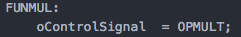
\includegraphics[width=1\textwidth]{controlfunc.png}
	\caption{Mapeamento de \textit{FUNMUL} para \textit{OPMULT}.}
	\label{fig:controlfunc}
\end{figure}

% todo : funjalr to opand ?

\subsection{Caminho de dados}
\label{subsec:datapath}

\subsection{Bloco de controle}
\label{subsec:control}

\subsection{Teste das novas instruções}
\label{subsec:testeisa}

\bibliographystyle{sbc}
\bibliography{relatorio}

\end{document}
